
\documentclass[a4paper,11pt]{article}
%在此可进行页面设置
%\textwidth=14cm
%\textheight=22cm
\usepackage{tikz}
\usetikzlibrary{mindmap,trees}
\usepackage{verbatim}

\usepackage{setspace}%使用间距宏包
\usepackage[76620]{MCMPackage}  %队号在这里填写
%\usepackage[XXX,nosheet]{MCMPackage}%这个参数形式可去掉summary sheet首页。
\problem{C}  %选题

\title{Energy Production}%在此插入论文标题
\date{\today}

%设置段落之间的距离,若不需要删除或者注释掉即可。
\setlength\parskip{.5\baselineskip}

%为了首行缩进
%\usepackage{indentfirst}
%\setlength{\parindent}{2em}

\makeatletter
\def\@cite#1#2{\textsuperscript{[{#1\if@tempswa , #2\fi}]}}
\makeatother

%设置参考文献的小上标

\begin{document}
%摘要
\begin{abstract}

\par For the sake of \textbf{\emph{Measuring the Evolution and Influence in Society's Information Networks}}, our idea is to set up a comprehensive model with plentiful properties of nodes which are consistent with the current states. Therefore, the concept of \textbf{\emph{Complex Network}} is introduced to depict information dissemination vividly. What's more, the \textbf{\emph{Twitter's Network Dataset}} is utilized to verify most of the models we build.


\par About Problem A, in order to \textbf{\emph{Explore the Information Flow}} and \textbf{\emph{Filter out Valuable Information}}, we establish the \textbf{\emph{Information Flow and Filter Model}}. Having considered the diversity in information media, the \textbf{\emph{Flexible Network Structure}} is explored to suit for the various types of information flow. Meanwhile, to gain a better information filter result, we create a filter consisting of ~$6$~ evaluation indexes. After theoretical preparation, we use the \textbf{\emph{Twitter's Network Dataset}} to establish Internet Information Flow and Filter Model for simulation. Finally, the coverage rate of information dissemination is equal to ~$96.7\%$~, after reaching the steady state of information dissemination.


\par As to Problem B \& C, based on the Information Dissemination Model, our assignment is to use the data to verify the \emph{\textbf{Reliability of the Model}} and \emph{\textbf{Predict the Future Data}}. We establish the \emph{\textbf{Network Evolution Model}} to imitate the dynamic network structure in a single medium. The \textbf{\emph{Average Euclidean Distance}} of the \textbf{\emph{real data}} and the \emph{\textbf{predicted data}} is ~$1.784$~, which stands for a good forecast result. After that, we take the model as the basis for the prediction of the Society's Information Network in $2050$. Without considering the emergence of new technologies, the cell phone usage is 51.34\%, which is the highest in the $4$ kinds of media. However, after making bold assumptions that the \emph{\textbf{Quantum Communication}} would be invented in $2035$, the share of the information medium will change dramatically, and the \emph{\textbf{Quantum Communication }} would be the main medium.

\par  When solving the Problem D \& E, we are required to analyze the Public Opinion Dissemination. We divide the network nodes into $3$ types: \textbf{\emph{Individuals, Opinion Leaders and Internet Marketer Group}}. And then we establish the \emph{\textbf{Public Opinion Dissemination Model}} to simulate the real situation of the public opinion dissemination, and draw the contrast curves of public opinion dissemination coverage rate before and after \textbf{\emph{Taking "PUSH" Operation}}. Finally, we screen out the effect factors of public opinion dissemination, and use the example of \textbf{\emph{President Obama's Nearly Opened Twitter}} to verify the stability of the model.


\par The accuracy and stability of our model are proved by simulation using the \emph{\textbf{Twitter's Network Dataset}}. Furthermore, the Information Dissemination Network Model can adapt to different types of media. By slightly adjusting the coefficients, we can apply this network model in various fields of information dissemination.


\textbf{Keywords: Information Dissemination Model; Dynamic Network Structure; Twitter's Network Dataset; Simulation \& Verification} 

\end{abstract}
\maketitle%插入标题
\thispagestyle{empty}%本页不遍页码

\newpage%另起一页插入目录
\thispagestyle{empty}%防止目录两页而出现一页带页码
\begin{spacing}{0.5}%%行间距变为single-space
\tableofcontents%目录
\maketitle
\thispagestyle{empty}
\end{spacing}

\newpage%另起一页书写正文
\pagenumbering{arabic}%开始编页码(阿拉伯数字)

\section{Introduction}
%In reference \cite{RefB}.%引用参考文献

\subsection{Background}
 
\par Nowadays, with the development of technology and the deterioration of environment, many countries, especially the Uinted States, began to value the clean and renewable energy, such as natural gas and electricity. Meanwhile, traditional energy, such as gasoline and coal, still plays an important role in economics. And it is obvious that the usage of the clean and renewable energy will support the future of mankind.
\par In the United States, an interstate compact is an agreement between two or more states. Frequently, these agreements create a new governmental agency which is responsible for administering or improving some shared resource such as a seaport or public transportation infrastructure.\cite{1} In 1970, the Western Interstate Energy Compact was formed, which was devoted to foster cooperation to develop and manage the nuclear technology. Recently, California, Arizona, New Mexico, and Texas wish to form a new interstate energy compact focused on increased usage of cleaner, renewable energy sources. 
\par A data file provides 50 years of data in 605 variables on each of these four states' energy production and consumption, along with some demographic and economic information. In order to inform a set of goals for the new interstate energy compact, we will analysize the data file and model.





\subsection{Problem Restatement and Analysis}
%这一部分写问题分析以及我们要解决的问题
\subsubsection{Part \uppercase\expandafter{\romannumeral1}}
\par For Problem A, in order to lay the foundation of analyzing , we are required to create an energy profile for each of the four states. Meanwhile, the profiles should be created on the analysis of the given data.

\par In regard with Problem B, 

\par It's closely followed by Problem C that asks for the forecast about the communication networks' relationships and attributes around the year 2050. 

\par Problem D requires us to explore how public interest and opinion can be change by applying the theories and concepts of information influence on networks. 

\subsubsection{Part \uppercase\expandafter{\romannumeral2}}
\par It is suggested in the Problem A that,

\par As for Problem B, 

\subsubsection{Part \uppercase\expandafter{\romannumeral3}}
\par On the basis of the analysis and models in the two parts before, we prepare the state profiles of 2009, our predictions towards energy usage and some recommendations on adopting goals for the energy compact.


\section{Assumption}
\begin{enumerate}%[(1)]
\renewcommand{\labelenumi}{(\theenumi)}
    \item In factor analysis, we suppose the corresponding valuables as the main factors when cumulative percentage is over 0.65 .
    \item Information network and evolution network are universal and suitable for each kind of media.
    \item The information network is affected  only by the factors that have been recognized.
    \item In the process of information dissemination, we assume that the network edge is directed.
    \item It is assumed that only the neighboring nodes will be affected.
    \item Information can only be transmitted from the source to the spread point, and it will not produce cross dissemination.
\end{enumerate}

%这里写模型假设


\section{Symbol Description}
%符号说明
In the section, we use some symbols for constructing the model as follows.

\begin{center}
\begin{tabular}{cc}%r 表示表格内文本右对齐;c表示居中对齐;l表示左对齐;| 表示竖铅直线
    \toprule[2pt]
    \textbf{Symbol} & \makecell[c]{\textbf{Description}}\\
    \hline
$R$&The correlation coefficient matrix of natural gas, electricity, fuel oil and coal coke.\\ 
$\lambda_i$&The eigenvalue of R, i = 1, 2, 3, 4.\\
$U$&The Eigenvector matrix for the eigenvalues of R.\\ 
$A$&The factor loading matrix.\\
$f_i$&Factor, i = 1, 2.\\ 
$w_1$&The weight of natural gas.\\ 
$w_2$&The weight of electricity.\\ 
$w_3$&The weight of fuel oil.\\ 
$w_4$&The weight of coal coke.\\ 
$\eta_1$&The proportion of renewable energy in total energy.\\
$\eta_2$&The proportion of different sector in renewable energy usage.\\
% $T_n$&The discrete time series of the node checking information.\\ 
% $p_{in}$& The probability of ~$Node~i$~ to check information at the moment of $T_n$.\\
% $q_{in}$&The probability that information is able to continue to spread\\
% $\lambda_i$&The probability of node's retransmission or comments after receiving the message.\\
% $N_n$& The number of nodes that have received information at the moment ~$T_n$~\\
% $Q_n$& The number of nodes that have received information at the moment ~$T_n$~\\
% $\gamma_i$& The new attention degree of a certain node in the unit time ~$\Delta t$~\\
% $D_i$&The degree of ~$Node~i$~\\
% $C_i$&The clustering of ~retransmission~$Node~i$\\
% $L_{ij}$&The shortes path length of ~$Node~i$~ and ~$Node~j$\\
    \bottomrule[2pt]
    %以下两条指令此处不用
    %\caption{表格标题}
    %\label{标签名}%便于交叉引用
\end{tabular}
\end{center}



\emph{P.S: Other symbol instructions will be given in the paper.}







\section{Problem A : Energy profile for each of the four states}
\par Factor Analysis is a multivariate statistical analysis method, which is based on the internal dependencies of the correlation matrix of the indicator. It attributes some of the variables that have complex relationship to a few irrelevant factors.\cite{2} We will use this method to deal with problem A in the section.

\subsection{MSN Analysis}
\subsubsection {MSN character analysis}

\par  By observing the given data and acquiring knowledge from reference materials, we can conclude that the MSNs are usually five-character codes, and the three parts of the characters generally represent the following meanings.

\begin{itemize}
    \item First and second characters: describes an energy source (for example, NG for natural gas, MG for motor gasoline);
    \item Third and fourth characters: describes an energy sector or an energy activity (for example, RC for residential consumption, PR for production);
    \item Fifth character: describes a type of data (for example, P for data in physical unit, B for data in billion Btu).	\cite{3}
\end{itemize}

\par As described above, the first part and the second part of the MSN code represent for certain specific meanings. However, in our analysis process, we are more concerned about the general classification of these MSN codes. 

\begin{figure}[h]%[!hptb] 
    \centering 
    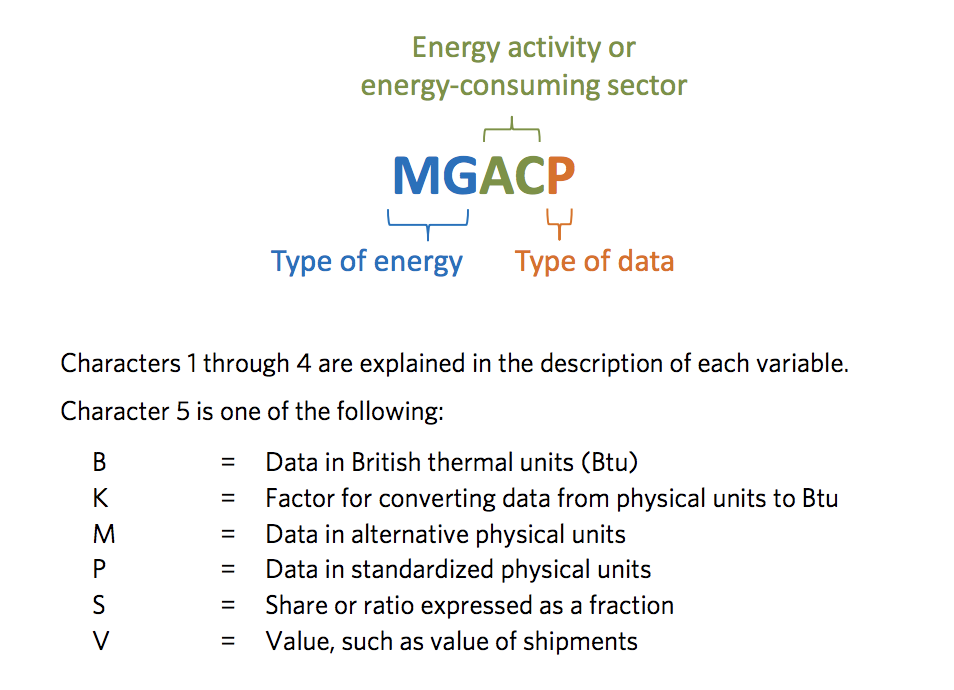
\includegraphics[width=0.8\textwidth]{./Pic/msn_5.png}
    % 图片标题
    \caption{The meaning of a MSN code, emphasizing the fifth character. Reference \url{https://www.eia.gov/state/seds/sep_use/notes/use_a.pdf}}
    \label{fig:msn_5}  
\end{figure}
\par We also found that the fifth character has six values at most, which can be seen in figure \ref{fig:msn_5}. Thus we start to focus more on the analysis of the fifth character. After comparing the units of the six and calculating, we find the relationship between these six symbols are
\begin{equation}
    B=KP~~~~~,~~~~~V=BD
\end{equation}

\par From the equation we can get the conclusion that B is a key factor between the two equations and can build a connection between them. And we find that all MSNs whose fifth character is B have the same unit Billion Btu, which can be an excellent representative of the MSNs who have the same prefix. So we filter the 605 MSNs and find 215 MSNs' suffix is B. At this stage we have reduced the 605 kinds of MSNs into 215. Every kind of the 215 MSNs contains several MSNs with different suffix but the same prefix.

\subsubsection {MSN classification analysis}

\begin{figure}[!h]%[!hptb] 
    \centering 
    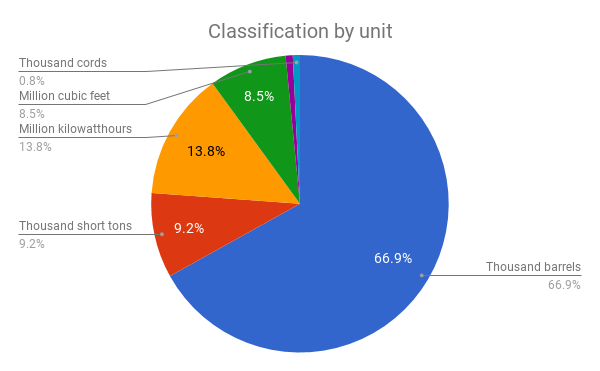
\includegraphics[width=0.8\textwidth]{./Pic/classification_by_unit.png}
    % 图片标题
    \caption{Classification by unit in the suffix P.}
    \label{fig:classification_by_unit}  
\end{figure}

\par In order to classify the 215 MSNs more clearly, we look into everyone of the division and find that a large percent of the kinds have the suffix P, which represents the standardized physical units. Physical units naturally represents for the energy classification in the real physical world, and there are mainly 4 kinds of standardized physical units in the data set as can be seen in figure \ref{fig:classification_by_unit}, so it is reasonable to classify the data into 4 groups according to the units.
\par According to the analysis above, we suppose the four units as the following representatives.
Thousand barrels: fule oil
Thouesand short tons: coal coke
Million kilowatthours: electricity
Million cubic feet: natural gas
\par Besides, there are many relationships among MSNs. According to the Formula in the Table A1.Consumption Variables,\cite{4} we remove variables that can be obtained by addition and subtraction of other variables, so that we can avoid the repeat of variables when we calculate the correlation coefficient matrix. 
\par In probem A, we will analysize the data processed in 2009, and obtain the 2009 energy profile for each of the four states.

\subsection{Factor Analysis Model}

\paragraph{4.2.1 Factor loading matrix}
\textrm{\\}
\par Hear, we take California as an example to show the process of modeling. By using the data processed, we obtain R, which is the correlation coefficient matrix of natural gas, electricity, fuel oil and coal coke.
\begin{equation}
    \centering
R=\begin{pmatrix} 1 & -0.389890 & 0.432474 & -0.004734 \\ -0.389890 & 1 & -0.094940 &-0.158034 \\ 0.432474 & -0.094940 & 1 & -0.016881 \\ -0.004734 & -0.158034 & -0.016881 & 1\end{pmatrix}
\end{equation}


\par Then we can obtain 
\[
\lambda_1=1.638729, \lambda_2=0.454611, \lambda_3=1.089176, \lambda_4=0.817484
\]
which are the eigenvalue of R.
\par Meanwhile, we obtain the eigenvector matrix for the eigenvalues of R.
\begin{equation}
    \centering
U=\begin{pmatrix} -0.666575 & 0.728151 & -0.131346 & -0.090683 \\ 0.281798 & 0.050295 & -0.698391 & -0.655981 \\ -0.423756 & -0.393132 & 0.443861 & -0.684737 \\ -0.544701 & -0.559209 & -0.545881 & 0.304303\end{pmatrix}
\end{equation}
\par Simply, the overall percentage and cumulative percentage of eigenvalues are as follows.
\begin{table}[!hbp]
    \centering 
    \begin{tabular}{|c|c|c|}
\hline
Eigenvalue & Overall percentage & Cumulative percentage \\
\hline
$\lambda_1$=1.638729 & 0.409682 & 0.409682 \\
\hline
$\lambda_3$=1.089176 & 0.272294 & 0.681976 \\
\hline
$\lambda_4$=0.817484 & 0.204371 & 0.886347 \\
\hline
$\lambda_2$=0.454611 & 0.113653 & 1.000000 \\
\hline
\end{tabular}
\caption{Percentage}
\end{table}
\par Therefore, the cumulative percentage of $\lambda_1$ and $\lambda_3$ is 0.681976 colse to 0.7.
\par According to assumption 1, the main factors are natural gas and fuel oil, the corresponding eigenvalues are $\lambda_1$ and $\lambda_3$. Then we take out their corresponding eigenvectors from U, and we can obtain the factor loading matrix
\begin{equation}
    \centering
A=\begin{pmatrix} 0.856438 & -0.145463 \\ -0.657207 & -0.429761 \\ 0.673909 & -0.408171 \\ 0.138447 & 0.846592\end{pmatrix}
\end{equation}
the first row of A is
\begin{equation}
    \centering
\sqrt{\lambda_1} \times U[ ,1]
\end{equation}
the second row of A is
\begin{equation}
    \centering
\sqrt{\lambda_3} \times U[ ,3]
\end{equation}

\paragraph{4.2.2 Factors and weights}
\textrm{\\}
\par According to the factor loading matrix A, we can get the factor analysis model is
\begin{equation}
    \centering
     natural gas=0.856438 \times f_1-0.145463 \times f_2
\end{equation}
\begin{equation}
    \centering
 electricity=-0.657207 \times f_1-0.429761 \times f_2
\end{equation}
\begin{equation}
    \centering
 fuel oil=0.673909 \times f_1-0.408171 \times f_2
\end{equation}
\begin{equation}
    \centering
coal coke=0.138447 \times f_1+0.846592 \times f_2
\end{equation}
\par The definition of the weight of variables is\cite{5}
\begin{equation}
    \centering
w_i=\frac{ \theta_i }{ \sum_{i=1}^{4}\theta_i } \times 100\%
\end{equation}
\begin{equation}
    \centering
\theta_i=A[i,1] \times 0.409682+A[i,2] \times 0.272294+A[i,3] \times 0.204371+A[i,4] \times 0.113653
\end{equation}

\par Therefore, we can obtain the the weight of natural gas, electricity, fuel oil and coal coke.

\[
w_1=25.640737\%, w_2=25.775307\%, w_3=23.682713\%, w_4=24.901242\%.
\]

\paragraph{4.2.3 Analysis of the factor analysis model}

\textrm{\\}
\par From the point of the factor analysis model, we can easily find that $f_1$ is a positive factor for natural gas, fuel oil, coal coke, and a negative factor for electricity. Meanwhile, $f_2$ is a positive factor for coal coke, and a negative factor for natural gas, electricity, fuel oil. 
\par By the model above, we can obtain the weights of variables of the four states as follows.
\begin{figure}[!hptb] 
    \centering 
    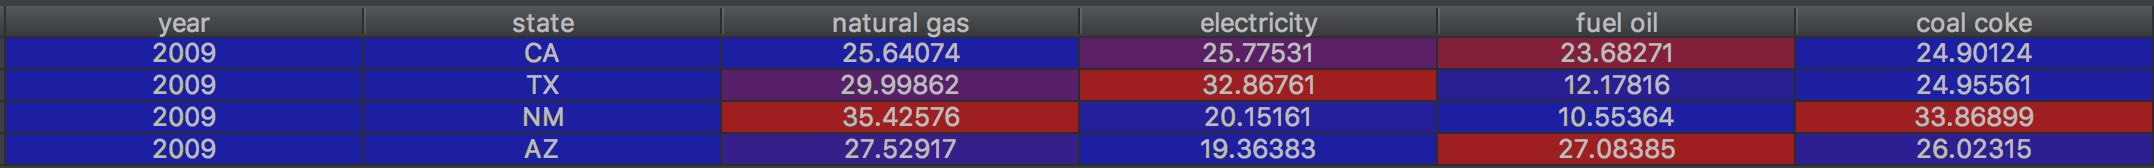
\includegraphics[width=1.0\textwidth]{weights.jpg}
    \caption{Weights of variables of the four states}
\end{figure}
\begin{figure}[!hptb] 
    \centering 
    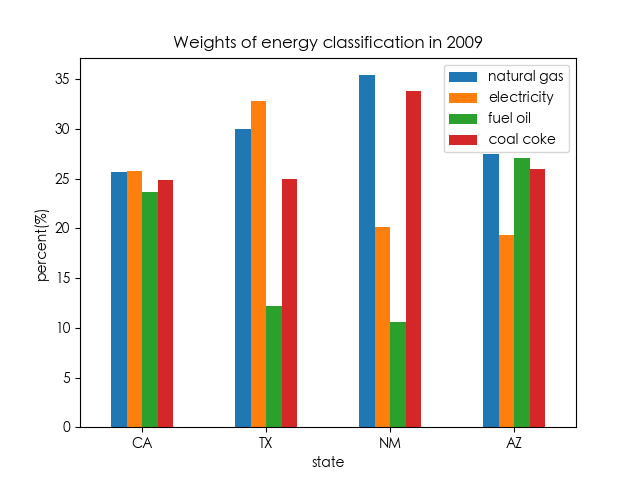
\includegraphics[width=0.8\textwidth]{1-1.png}
    \caption{Weights of energy classification in 2009}
\end{figure}
According to Figure 4, the contribution rates of four energy are very close in California. But in New Mexico and Texas, natural, electricity, and coal coke are main energy, because the addition of their contribution rates is over 85\%. And in Arizona, the contribution rate of electricity is less than the other energy. 

\paragraph{The attributes of each part of the network}
\textrm{\\}

\begin{itemize}
\item Network structure attribute: the characteristic attributes of different networks are embodied in the different number of nodes and different number of edges. Node degree is different, resulting in the transmission efficiency of the node is different, the speed of the network is different.
\item Node attribute: the degree of nodes is different, resulting in the probability of the node to receive the message is different, the probability of the spread of the message is also different.
\item Attribute of the information itself: the attribute of information itself is mainly reflected in the importance of the information and the correlation degree of the information.
\end{itemize}

\subsubsection{Example of Information Flow Network Model (Internet)}
\par In order to better explain the theoretical model we have constructed, we build an example model, which takes the Internet as a single media of dissemination.
\paragraph{Construction of realistic network model}
\textrm{\\}
\par After analyzing the theoretical model, we will set up the concrete social's information flow model in Internet.
\par We establish a social network, which is a \textbf{\emph{directed}} graph
\begin{equation}
G_I=(V_I,E_I)~~~~~~~\forall  v_I,u_I\in V_I , \forall e_I=(u_I,v_I)\in E_I
\end{equation}
where ~$v_I$~ and ~$u_I$~ are the nodes of ~$G_I$~, representing the \emph{people or group in society network}. And ~$e_I$~ stands for the edge, representing the \emph{transmission route between people or groups}. Meanwhile, the ~$e_I$~ can also represent that ~$u_I$~ can receive information from ~$v_I$~, the same as ~$u_I\leftarrow v_I$~. We also define ~$\mid V_I\mid$~ as the number of people or groups and ~$\mid E_I\mid$~ as the total number of transmission route.
\par The discrete time series of the node checking information is ~$T_n,n=1,2,3...$~, the probability of ~$Node~i$~ to check information at the moment of ~$T_n$~ is ~$p_{in},i=1,2,3...,\mid V_I\mid$~; ~$p_{in}\in [0,1]$~ is an independent random variable.
\par Assuming that at the moment of ~$T_n$~, the node has received a message, then the probability that information is able to continue to spread is ~$q_{in}$~
\begin{equation}
q_{in}=p_{in} \times [(1-(1-\lambda_{i})^m)/e^{\alpha +\beta}]
\end{equation}

where 
\begin{itemize}
\item ~$\lambda_{i}$~ is influenced by the information attribute factors and the subjective factors of nodes, standing for the probability of node's retransmission or comments after receiving the message.
\item ~$m$~ represents the ~$Node~i$~ has accepted the cumulative number of information at the moment of ~$T_n$~. 
\item ~$\alpha$~ is the cumulative credibility of information sources. ~$\beta$~ is the cumulative number of strong relationship of information sources.
\end{itemize}

\par In the model we have established, the node is human. Under this circumstance, if we need to study node attribute, we have to take into account different types of people. The biggest difference among the different groups is the age structure. Different nodes have different age structures, so there are different node attributes. 



\par We find that not only the attributes of the nodes can affect the propagation of information, but also the properties of the network structure will play a very important role. Different times have different modes of transmission, in the 1870s, newspapers were delivered by trains and stories were passed by telegraph; in the 1970s, when televisions were in most homes; in the 1990s, when households began connecting to the early internet; in the 2010s, when we can carry a connection to the world on our phones. The main difference between different modes of transmission is the spread speed of the media, which can affect the structure of the network. Therefore, we have to take the transmission modes into account. 

\par In this example,the information source is people or groups, spreading the information. The information dissemination has two ways to spread it. One is the \textbf{\emph{interpersonal communication}}, the other is the \textbf{\emph{across-platform communication}}. The former method is oral communication. The latter includes different ways.



\subsection{Information Filter Model}
\par The presence of incorrect and misleading content on the Web can have serious consequences for people who increasingly rely on the internet as their information source for topics such as health, politics, and financial advice\cite{RD}. Under these circumstances, we have to establish a model of information filter to screen for real, valuable messages.
\par In order to solve this problem, we set up an information value evaluation model. The schematic diagram of evaluation index classification is Figure \ref{fig:The_schematic_diagram_of_evaluation_index_classification} as follows.


\begin{figure}[h]%[!hptb] 
    \centering 
    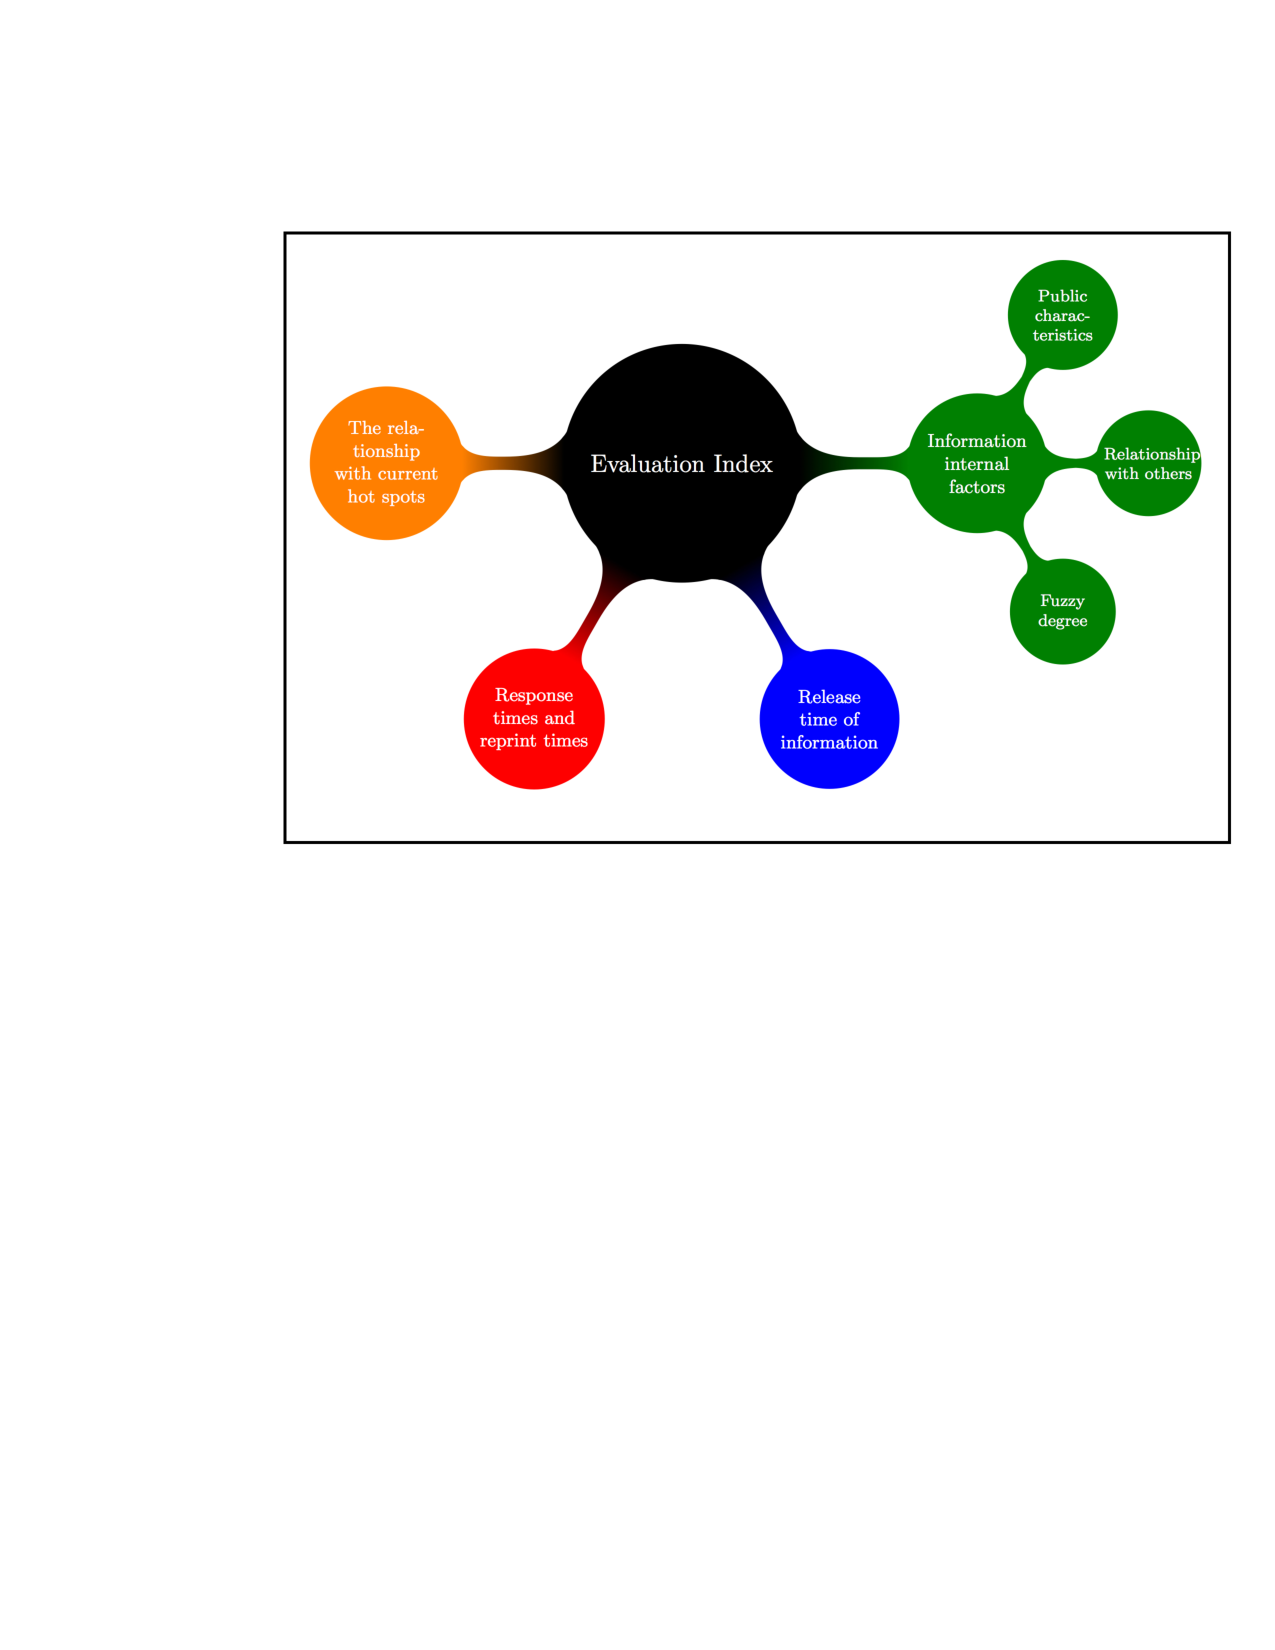
\includegraphics[width=0.6\textwidth]{./Pic/The_schematic_diagram_of_evaluation_index_classification.pdf}
    % 图片标题
    \caption{The schematic diagram of evaluation index classification. The center node has 4 screening indexes, each index has different subindexes.}
    \label{fig:The_schematic_diagram_of_evaluation_index_classification}  
\end{figure}

\par After selecting good evaluation indexes, we will quantify the various evaluation indexes to measure the information and screen out the valuable information. The screening index calculation formula is as follows.
\begin{equation}
\omega=e^{-a(t-t_s)} \times b _i \times b _j \times b _k \times b_h
\end{equation}
where the ~$b _i,b _j,b _k$~ are the independent random variable, ~$b _i$~ is the relationship degree with current hot spots, the ~$b _j$~ is the degree of public concern about the information, and ~$b _k$~ is the response degree. What's more,~$b_h$~ represents the  information internal factor index. ~$t$~ is the current time, ~$t_s$~ is the release time. ~$a$~ stands for the time factor.
\par The formula above has 4 independent random variables. Because of the absence of specific screening data, we can not make a further analysis of the model. We can only give the preliminary model above.


\subsection{Renewable energy profile}

\par In the previous section, we have set up a good factor analysis model for energy classification. It dose help us build the profile of the states' energy, but it dosen't pay much attention to the difference between renewable energy and non-renewable energy. So in this part, we analyze the data set and give the profile of renewable energy in four states.
\subsubsection{Renewable energy usage percentage}
\par To get a preliminary understanding of the renewable energy usage in four states, we decide to get the proportion of renewable energy in total energy in the first step.

\par What's important is that, we find that there are some specific MSNs and formulas in the reference \cite{4} which can describe the usage of renewable energy clearly and precisely. MSN RETCB is a good example, which represents renewable energy sources total consumed in a state.
\par Then we search for the MSN in the given data and find every state have have this MSN. So this is indeed the representative MSN variable of the usage of renewable energy in every states. And then we find the TETCB MSN stands for the total energy consumed in a state. So we get the equation like this

\begin{equation}
    \eta_1=\frac{RETCB}{TETCB}
\end{equation}

\begin{figure}[h]%[!hptb] 
    \centering 
    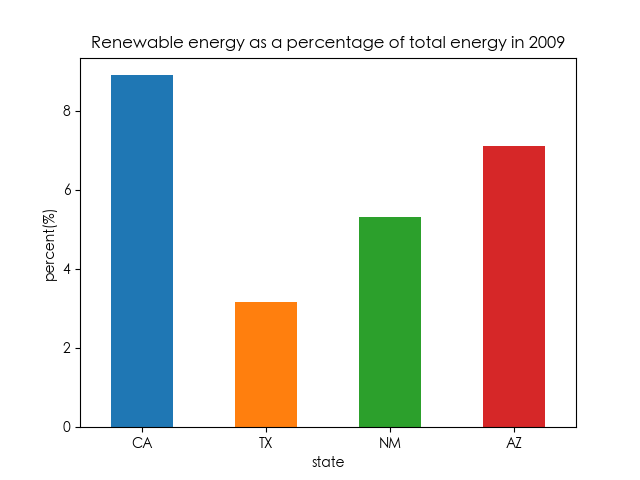
\includegraphics[width=0.6\textwidth]{./Pic/1-2.png}
    % 图片标题
    \caption{The proportion of renewable energy in total energy in four states in the year of 2009.}
    \label{fig:1-2}  
\end{figure}
\par After calculating with the formula, we get the results of $\eta_1$, which can be seen in figure \ref{fig:1-2}

\subsubsection{Renewable energy usage in different sector}
\par There are many factors that influence the usage of energy in a state. So it is reasonable to search for the situation of renewable energy usage in different sector in every state.
\par Similar to the previous section, we find that there are some MSNs that describe the renewable energy in certain sector and formulas that calculate for the value of it. Take transportation sector for example, MSN REACB stands for renewable energy sources consumed by the transportation sector, so the sector's percentage in renewable energy consumption can be calculated through the formula

\begin{equation}
    \eta_2=\frac{REACB}{RETCB} \times 100\%
\end{equation}

\begin{figure}[h]%[!hptb] 
    \centering 
    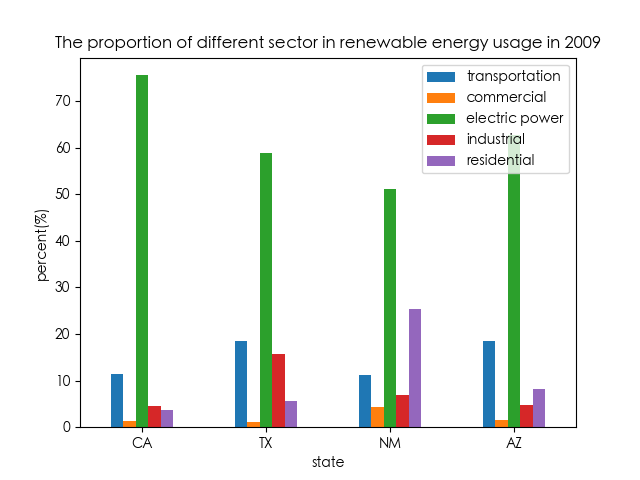
\includegraphics[width=0.6\textwidth]{./Pic/1-3.png}
    % 图片标题
    \caption{The proportion of different sector in renewable usage in four states in the year of 2009.}
    \label{fig:1-3}  
\end{figure}
\par After calculating with the formula, we get the results of $\eta_2$ , which can be seen in figure \ref{fig:1-3}






\section{Problem B : Profile evolution \& Energy usage comparison among four states}

\par In order to verify our model's reliability, we have to build a short term prediction model to predict the information communication situation for today by using data from the past, and compare them with today's reality.
\subsection{Short Term Prediction Model of Information Dissemination}
\par In this chapter, we first describe the theoretical model of the building, and then build a realistic model of information dissemination.
\subsubsection{Model preparation}
\paragraph{Node distinction}
\text{\\}
\begin{itemize}
\item Isolated node: there is no connection with other nodes at a certain time, and the next moment it may be linked to other nodes in a certain probability.
\item Isolated cluster: there is no connection with other clusters at some point in the next moment, which may be related to other clusters at a certain probability. And there are interconnected nodes in the cluster.
\item Large scale network cluster: cluster network is composed of many nodes or clusters, and there are direct or indirect links between nodes or clusters in the network.
\end{itemize}
\textbf{\emph{Assuming there is no absolute isolated node or cluster, any node or cluster is directly or indirectly connected with other nodes or clusters.}}



\subsubsection{Realistic network model construction}
\par Next, we build the realistic network model by steps.
\paragraph{(1) Constructing a dissemination network}
\text{\\}
\par We define that there are $N_r$ nodes and ~$M_r$~directed edge in the network. Meanwhile, we classify the nodes according to the node's own attribute and introduce the influence factor ~$\gamma _i$~, which would change with the change of the node itself. The ~$\gamma _i$~ represents the new attention degree of a certain node in the unit time ~$\Delta t$~.

\begin{equation}
\gamma _i=\frac{\Delta D_i}{\Delta t}
\end{equation}
\emph{where ~$D_i$~ stands for the degree of Node ~$i$~.}
\paragraph{(2) Adding the new people or group to the network}
\text{\\}
\par In each of the identified time series, the new node has two different ways to join the network.
\par One is establishing the connection relationship with the existing node freely. The probability of being associated with an already existing node is ~$p_i$~,
\begin{equation}
p_i=\frac{D_i+\gamma _i}{{\sum\limits_{i=0}^{N_r}}(D_i+\gamma _i)}
\end{equation}
\par The other is receiving the invitation, in accordance with the principle of common neighbor selection node to establish a connection. After the connection is established, according to the principle of preferential connection, the node will connect with the other nodes. 
\par The probability of connecting with the node ~$i$~ is ~$q_i$~, 
\begin{equation}
q_i=\lambda \beta _i+(1-\lambda ){\frac{{{D_i} + {\lambda _i}}}{{\sum\limits_{i = 0}^{{N_r}} {({D_i} + {\lambda _i})} }}}  
\end{equation}
where ~$\lambda\in {0,1}$~ stands for whether the node is invited. If not, ~$\lambda$~ taken ~$0$~, ~$\beta _i \in [0,1]$~ represents the probability of common adjacent nodes to promote the evolution.

\begin{equation}
\beta_i={\frac{g_{ij}}{G}}
\end{equation}

where ~$g_{ij}$~ stands for the number of having same neighbor between ~$Node~i$~ and ~$Node~j$~; ~$G$~ is the total neighbor number of ~$Node~i$~.
\paragraph{(3) Adding the new relationship to the network}
\text{\\}
\par For the existing nodes in the network, the probability of the link between the two nodes is ~$O_i$~,


\begin{equation}
{O_i} = ({\beta _i} + \frac{{{D_i} + {\lambda _i}}}{{\sum\limits_{i = 0}^{{N_r}} {({D_i} + {\lambda _i})} }})/2
\end{equation}



where ~$\beta_i$~ is the probability of common adjacent nodes to promote the evolution.





\paragraph{(4) Determine the upper limit of the relationship}
\text{\\}
\par Taking into account the actual factors, people's energy is limited. So there is an upper bound on the degree of the node. Before a degree does not reach the ceiling ~$I$~, the broken link probability between nodes is very small.
\par We assume that ~$k$~ is the number of other nodes, which are followed by a certain node. Then the probability of breaking one link is ~$Z_k$~,

\begin{equation}
{Z_k}=1-\lambda \beta _k+(1-\lambda ){\frac{{{D_k} + {\lambda _k}}}{{\sum\limits_{k = 0}^{{N_r}} {({D_k} + {\lambda _k})} }}}=1-q_k
\end{equation}



\paragraph{(5) Calculation of model evaluation index}
\text{\\}
\par In order to network structure, we ought to select several evaluation index. After choosing, the calculation formulas of model evaluation index are as follows:
\begin{equation}
AD=\frac{1}{N}{\sum\limits_{i}^{}}{K_i}
\end{equation}
where the ~$AD$~ stands for the average degree, ~$K$~ is the degree of nodes.
\begin{equation}
L=\frac{1}{n(n-1)}{\sum\limits_{i+1}^{}}{d_{ij}}
\end{equation}
where the ~$L$~ is the average path, $n$ is the number of nodes, and $d_{ij}$ is the shortest distance.
\begin{equation}
C_i=\frac{2l_i}{k_i(k_i-1)}{\sum\limits_{i+1}^{}}{d_{ij}}
\end{equation}
where ~$C_i$~ represents for the average clustering, ~$K_i$~ is the degree of ~$Node~i$~ and ~$l_i$~ is the actual variable between the adjacent points of the ~$Node~i$~.











\subsection{Model Simulation Process}
\par When the initial number of nodes is much smaller than the size of the final network, we are convinced that the number of initial nodes has no influence on the evolution of the network. So we chose the initial number of nodes is ~$3$~, and these ~$3$~ nodes constitute a complete graph. Meanwhile, We define a time period. In this period of time, we will add several nodes to the network randomly (up to no more than 10). The probability of being invited to joining the network and joined the network spontaneously is both 50 percent.
\par After joining the network, the newly added nodes are connected with the nodes which already exist in the network according to the probability of ~$p_1$~ and ~$p_2$~. In each time period, for the nodes which have already existed in the network, connect two unlinked nodes in accordance with the probability of ~$q_1$~, break the edge in accordance with the probability of ~$q_2$~.
\par In order to find the answer, we need to continue fitting and determine the value of ~$p_1, p_2, q_1, q_2$~. For simplicity, we assign fixed values to the ~$p_1$~and ~$p_2$~ after a small range of tests. Futhermore, in the subsequent simulation, the ~$p_1$~and ~$p_2$~ will be considered as fixed values.
\par We select the reference index is the average degree ~$AD$~ of the network, and then use the \textbf{\emph{least squares method}} to take regression analysis, determining the parameters which have the smallest error .
\par The specific process of model simulation is

\begin{enumerate}%[(1)]
\renewcommand{\labelenumi}{(\theenumi)}
    \item In the evolution of the network, when the network evolute to a state where has the same size with the existing referenced network, we mark this time as an observation point. At the end of evolution, we would compare the measured values of these observation points with the actual indicators of the existing reference network, and calculate the \textbf{\emph{square sum of errors}}.
    \item Erase data, and repeat the first step of the experiment 100 times.
    \item After determining the parameters, we would make five simulation in each network size comparison point. And then, make the calculation of the each index to obtain the average value and get the final simulation data.
\end{enumerate}

\subsection{Forecast \& Validation Results}
\par After the simulation of the model, we have obtained the data, and then compare it with the actual data. The results are as follows.
\subsubsection{Forecast Results}
\par Several results of forecast are listed in the Table \ref{tab:addlabel} as follows.

\begin{table}[htbp]
  \centering
  \caption{The Forecast Date of Information Network's Characterization (2010-2014)}
    \begin{tabular}{cccc}
    \toprule
    year  & simulate average degree & simulate average clustering & simulated ASPL \\
    \midrule
    2001  & 13.01939492 & 0.419213291 & 4.801293321 \\
    2002  & 16.19395812 & 0.429192399 & 4.56234903 \\
    2003  & 19.94393111 & 0.435029123 & 4.423443242 \\
    2004  & 21.49283818 & 0.441919291 & 4.39919291 \\
    2005  & 22.89182849 & 0.450203023 & 4.311232131 \\
    2006  & 24.19294829 & 0.458049292 & 4.19191011 \\
    2007  & 24.94812912 & 0.462838322 & 4.16991911 \\
    2008  & 25.39181938 & 0.46478866 & 4.156568507 \\
    2009  & 25.59182389 & 0.467667754 & 4.151586061 \\
    2010  & 25.89182383 & 0.47086898 & 4.14725192 \\
    2011  & 26.10592911 & 0.472843919 & 4.141046295 \\
    2012  & 26.34929111 & 0.473818239 & 4.139822779 \\
    2013  & 26.72394393 & 0.47581239 & 4.132812418 \\
    2014  & 27.12939219 & 0.478923844 & 4.110359 \\
    2015  & 28.12939321 & 0.481192393 & 4.098181283 \\
    \bottomrule
    \end{tabular}%
  \label{tab:addlabel}%
\end{table}%
\textbf{\emph{ASPL: average shortest path length}}


\par From the data we obtain above, the \emph{Average Euclidean Distance} is ~$1.784$~. 
\par From Table \ref{tab:addlabel} above, we find that under the condition of having errors, the growth of forecast data is relatively slow. Therefore, we can conclude that in the relatively stable society, the network structure is in the occurrence of slow evolution. Meanwhile, the network model we established can adapt to the change of time.


\subsubsection{Validation Results}

\par The forecast data and the real data comparison chart is drawn in the Figure\ref{fig:P2} as follows.

\begin{figure}[h]%[!hptb] 
    \centering 
    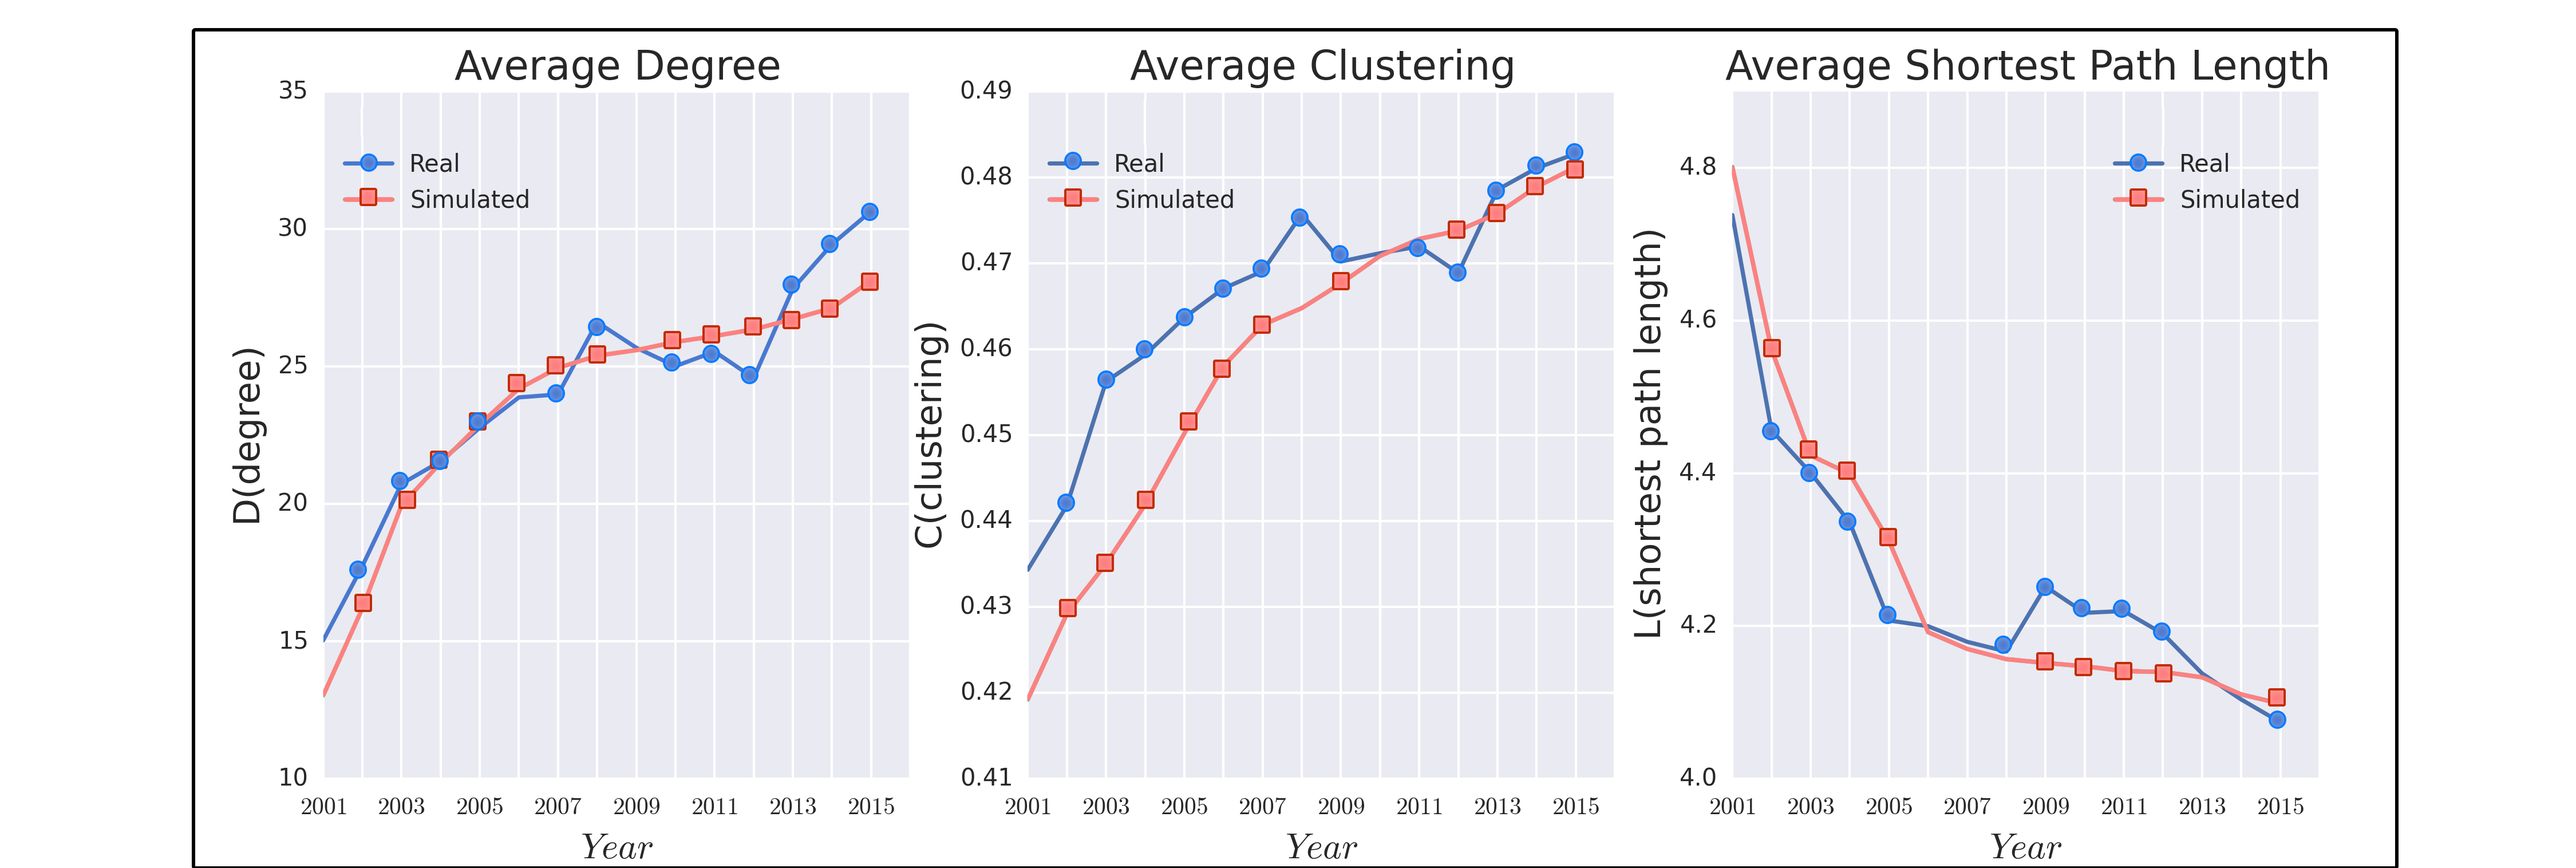
\includegraphics[width=1\textwidth]{./Pic/P2.jpg}
    % 图片标题
    \caption{Simulation results and actual data comparison chart. We compare the \textbf{\emph{Average degree, Average clustering and Average shortest path length}}.}
    \label{fig:P2}  
\end{figure}


\par From Figure \ref{fig:P2} above, and compare with the real data, with we can draw the conclusion: Under the condition of having errors, we believe that the simulation data and the real data fitting degree are very high, the changing trends of various indicators are the same. Therefore, as far as we are considered, the model is reliable and can predict the change of network structure in a short time.



\section{Problem C : Long Term Network Evolution Model}
\par The change of information propagation model is divided into the slow change of the short time and the significant change of the long time. If the new revolutionary means of communication would be invited, the information dissemination model will be a complete change. We also need to set up an evolution model to predict the long time changes after the short information transmission is predicted.

\subsection{Model building}
\par In order to measure the change of information media with time, we need to find an index. After analyzing the historical data and the network structure, we define the \textbf{\emph{network dissemination efficiency}} as the main index of the model, meanwhile, analyze it.
\par Through the analysis of the data, we find that in the emergence of new communication media, the usage rate of old communication media will be gradually reduced, but only a few communication media's usage rate tend to be 0, such as the telegraph. The remaining communication media will exist in the society according to a certain proportion, and affect our society in accordance with a certain proportion.
\par In this question, we use the ~$E$~ to represent the dissemination efficiency of the network. 

\begin{equation}
E=\sum a_kE_k 
\end{equation}
where the ~$E_k$~ is the dissemination efficiency of the network of the ~$k^{th}$~ medium.

\subsection{The bold assumption of future communication technology}
\par \textbf{\emph{Innovative ideas require bold assumptions.}}Our analysis of the evolution of information media from 1870s to 2010s found that the emergence of new media will greatly change the pattern of information dissemination. 

\par The following Figure \ref{fig:04} is the timeline of the main information dissemination media changes.
\begin{figure}[h]%[!hptb] 
    \centering 
    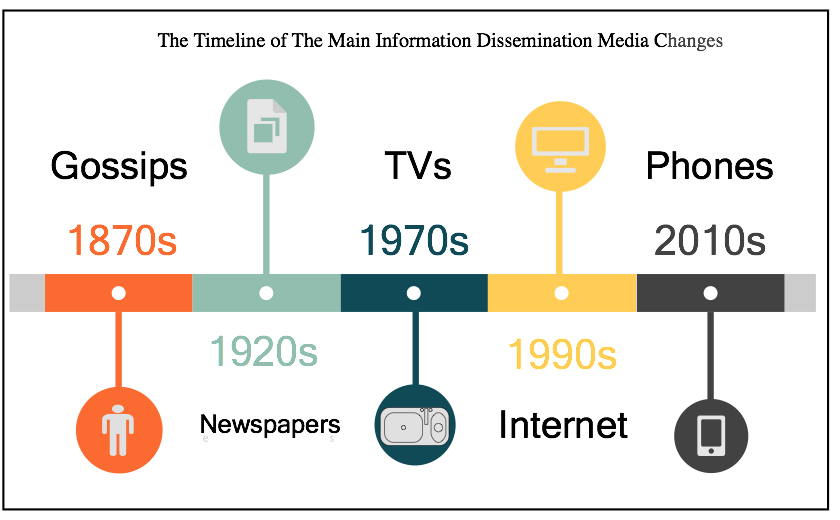
\includegraphics[width=0.55\textwidth]{./Pic/04.png}
    % 图片标题
    \caption{The timeline of the main information dissemination media changes}
    \label{fig:04}  
\end{figure}

\par Under these circumstances, we are fully convinced that new information media is likely to be invented before the 2050. After consulting the relevant information\cite{RH}, we found that \textbf{\emph{Quantum Communication}} is likely to go on the stage of history. 

\par The definition of \textbf{\emph{Quantum Communication}} is the high performance communication using the quantum effect under the condition of physical limit. Quantum communication has many advantages as follows:

\begin{itemize}
\item Quantum cryptography provides a new method for absolutely secure communication.
\item Quantum Communication with good anti-interference does not depend on the transmission medium feature.
\end{itemize}
\par Because quantum communication has so many advantages and its research is also smooth, we boldly assume: before 2050, the quantum communication will come into being. Meanwhile, taking into account the process of quantum communication and the difficulty of commercial use, we assume that in ~$2035$~, the quantum communication will be officially entered the commercial market.




\subsection{Model solving}
\par We collect the data of the proportion of various media frome 1990 to 2015, and bring them into our model to solve. The result are as follows.

\par The lift figure above is the fitting result of date from 1990 to 2015\cite{RK} of the network effciency. The right  pie chart is the proportion of different information dissemination media (around 2050), from which the phone and the internet will become the most popular information dissemination media. Meanwhile, the radio, TVs and newspaper will gradually die out.


\begin{figure}[!h]
  \centering %使得插入的照片居中显示
  \begin{minipage}[t]{.49\linewidth}
   % \framebox{Text}
  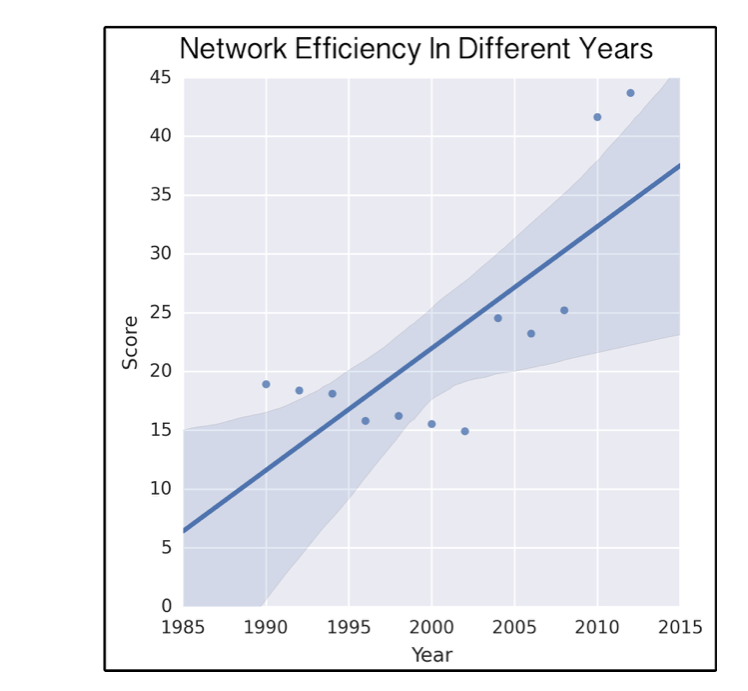
\includegraphics[width=1\textwidth]{./Pic/P3_.png}
  \caption{The Network Effciency in Different Years (1990-2015)}
  \end{minipage}
  \begin{minipage}[t]{.49\linewidth}
  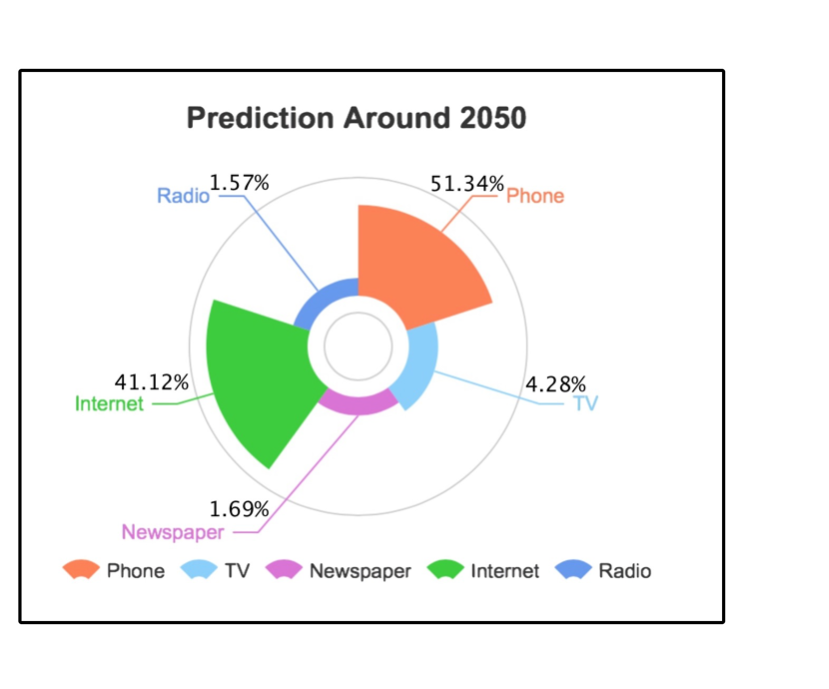
\includegraphics[width=1\textwidth]{./Pic/P3.png}
   %\framebox{Text}
  \caption{The Proportion of Different Information Dissemination Media Pie Chart (around 2050).}
  \end{minipage}
\end{figure}


\par The life line graph is the proportion of different information dissemination media around 2050 (\textbf{\emph{assume there is no new information dissemination technology appearing}}).  Left of the Dashed Line shows the real data collected online,while right display the predicted data.

\begin{figure}[!h]
  \centering %使得插入的照片居中显示
  \begin{minipage}[t]{.49\linewidth}
   % \framebox{Text}
  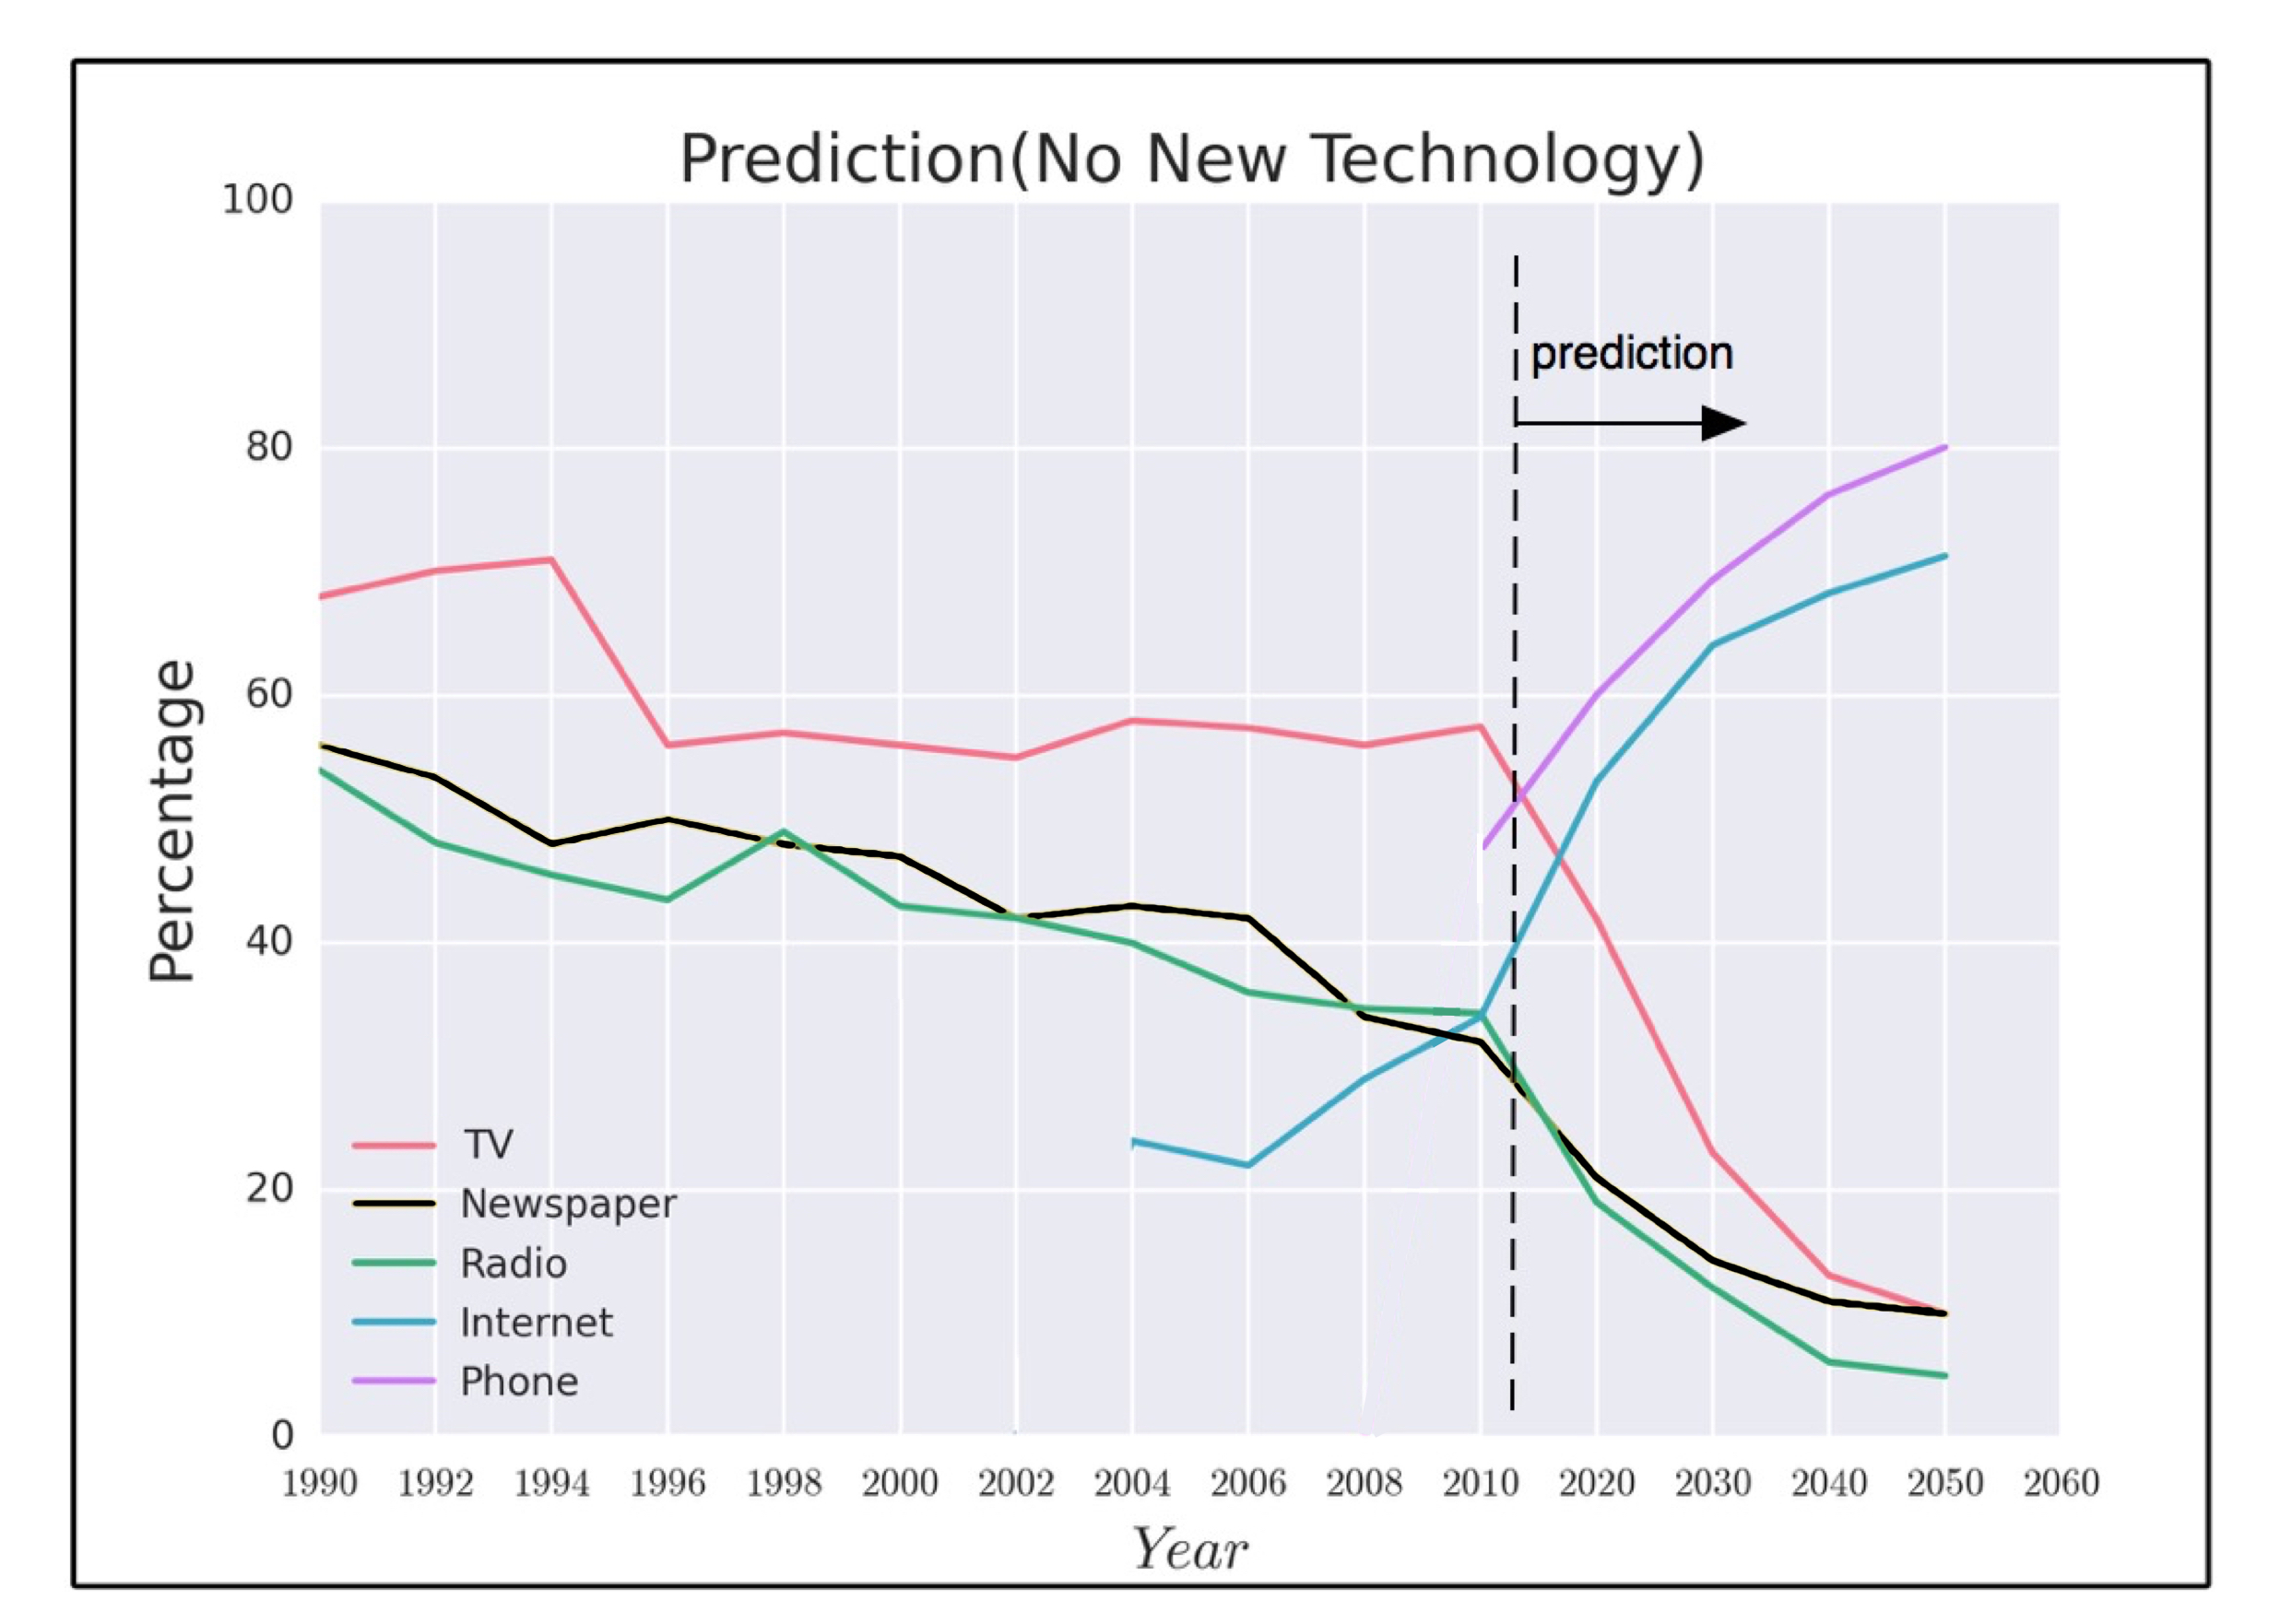
\includegraphics[width=1\textwidth]{./Pic/P3_21.jpg}
  \caption{The Forecast Curve of Different Media Using Proportion (No New Technology)}
  \end{minipage}
  \begin{minipage}[t]{.47\linewidth}
  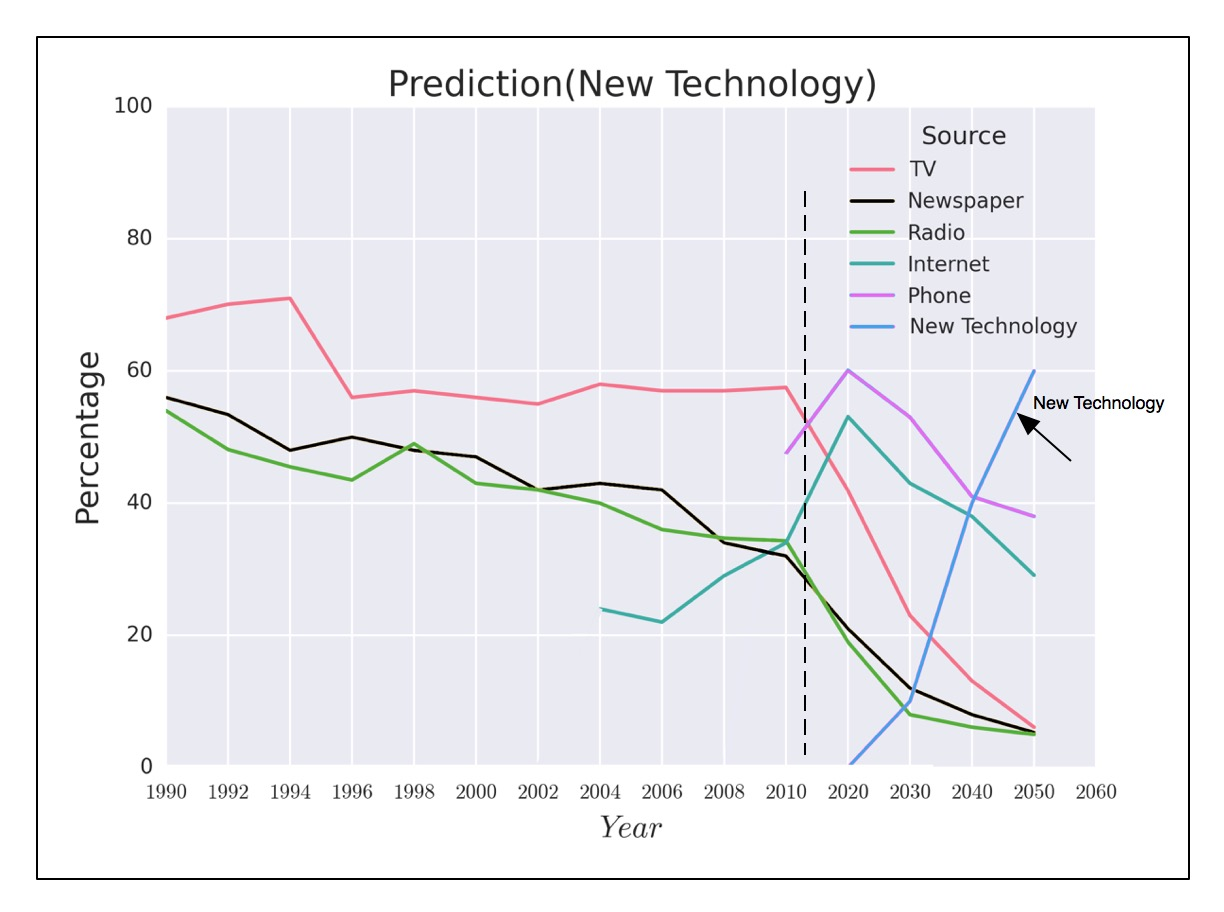
\includegraphics[width=1\textwidth]{./Pic/P3_22.jpg}
   %\framebox{Text}
  \caption{The Forecast Curve of Different Media Using Proportion (Invent New Technology)}
  \end{minipage}
\end{figure}


\par The right line graph is the proportion of different information dissemination media around 2050 (\textbf{\emph{assume there has new information dissemination technology appearing}}). Left part chart of the Dashed Line shows the real data collected online, while the right one displays the predicted data. The line which is pointed represents the time that the new technology turning up in the future which tends to influence the society.

\par We use the data obtained from the ITU to predict the condition of information dissemination media in 2050, as the same time, we also get the data verify the reliability of the model. Not only did we obtain the data based on the prediction of the emergence of new technology, but also through access to relevant information, we can boldly gain the date based on have a new technology coming into being. The model is comprehensive and accurate.









\section{Problem D : Public Opinion Dissemination Model}
\par As we all know, information is not a constant when it spreads. Information will be changed with the spread. At the same time of information dissemination, the public opinion will come into being. In this chapter, we will study the mechanism of public opinion dissemination, and establish a model.
\par When constructing the model of public opinion, we believe that different people will have different influence on public opinion. The difference between the first model and this question is: when we construct the first model, we assume that the contribution rate of each node is the same, and the noise of information is not considered in the process of dissemination. However, in this chapter, we construct the network model of public opinion which has different nodes.
\par We can divide the network nodes into the three different types.

\begin{itemize}
\item Individuals: People or group.
\item Opinion Leader: Determine the nature of the event in the network, and predict the future trend of the event.
\item Internet Marketer Group: Internet Marketer Group is a certain scale of the people. They have a certain influence on the event of large-scale nodes in the network. This kind of influence is not related to the distance.
\end{itemize}



\par In a network of public opinion, the schematic map of different typical nodes is as follows.


\begin{figure}[h]%[!hptb] 
    \centering 
    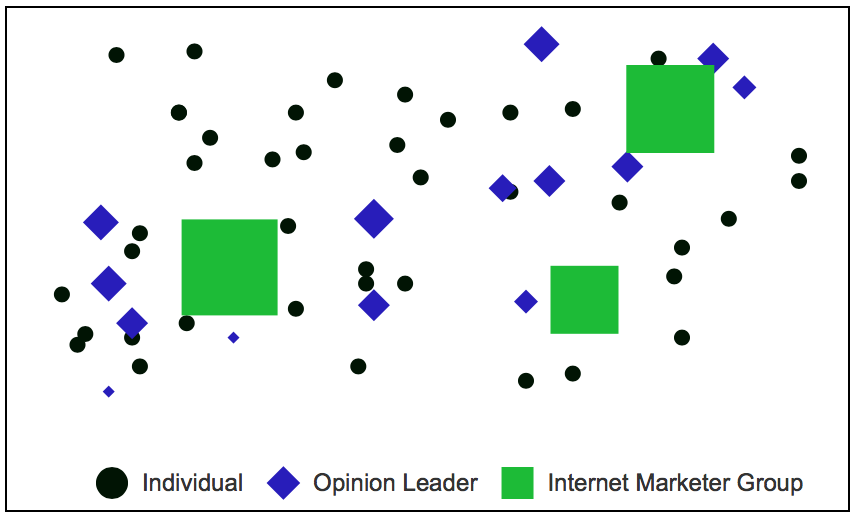
\includegraphics[width=0.7\textwidth]{./Pic/Unknown.png}
    % 图片标题
    \caption{Schematic diagram of different typical nodes distribution. The number of \textbf{Individuals} is the biggest, while the number of \textbf{Internet Marketer Groups} is smallest, but its influence is very big. Opinion leaders have a large influence and their quantity is not fixed.}
    \label{fig:Unknown}  
\end{figure}

\par After analyzing the classification of the network nodes, we use the Twitter's data we find to simulate.
\par On the basis of the network established in the first question, we select nodes with maximum degree, and take them as the \textbf{\emph{Internet Marketer Group}}. Meanwhile, we choose the nodes which have the second highest degree as the \textbf{\emph{Opinion Leader}}. We also define the other remaining nodes as the \textbf{\emph{Individuals}}.
\par After defining the nature of the network nodes, we use the \textbf{\emph{Information Network Flow Model}} to simulate this chapter's model.
\par After a period of time, we take the operation of \textbf{\emph{Push}} to network to improve the activity of the network information source, that is, to improve the success rate of information dissemination.
\par The results are shown in Figure \ref{fig:P4} as follows.


\begin{figure}[h]%[!hptb] 
    \centering 
    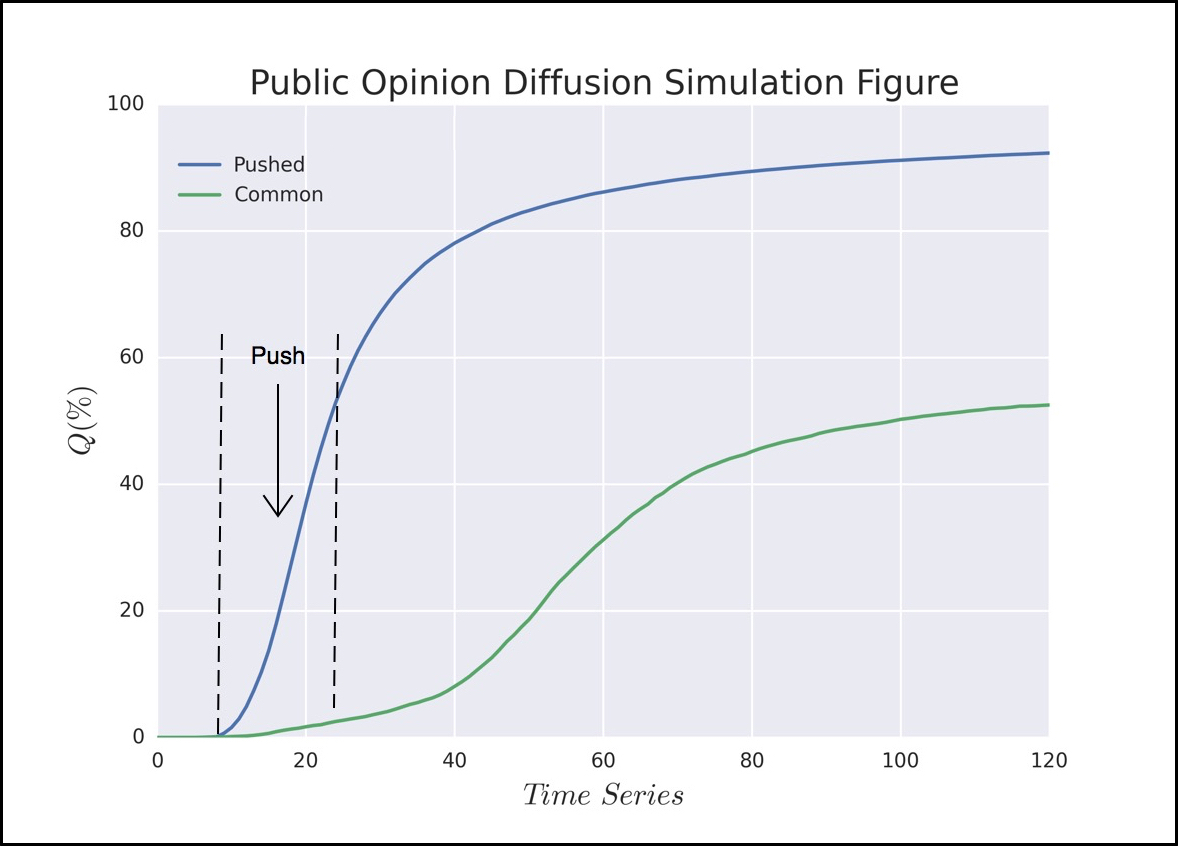
\includegraphics[width=0.5\textwidth]{./Pic/P4.jpg}
    % 图片标题
    \caption{Public opinion diffusion simulation figure.}
    \label{fig:P4}  
\end{figure}

\par In Figure \ref{fig:P4}, after taking operation of \textbf{\emph{Push}}, the message dissemination speed and the efficiency is greatly improved, showing the logistic growth, from which we can find that the operation of the network has a significant impact on the network. \textbf{\emph{Internet Marketer Group}} and \textbf{\emph{Opinion Leaders}} play an important role in the network of public opinion. Therefore, our \textbf{\emph{Public Opinion Dissemination Model}} is reliable and stable.









\section{Problem E : Analyze the Factors that Influence the Public Opinion Dissemination}
\par In the first question, we set up a model of public opinion dissemination. In this chapter, we will analyze the factors that influence the spread of public opinion. At the same time, a real society is analyzed.
\subsection{Influence Factors of Public Opinion Disseminate}
\par There are many factors that affect the spread of public opinion, and we choose the following ~$4$~ factors as the main factors.


\begin{enumerate}%[(1)]
\renewcommand{\labelenumi}{(\theenumi)}
    \item Information value

    The formula for calculating the value of information has been given in the first question. Information value can influence not only the speed of information dissemination, but also the public opinion. value of information is high, the probability of people receiving information and the degree of acceptance will be improved.


    \item People's initial opinions and prejudices

    Psychologists believe that humans are "cognitive misers"\cite{RE}. People always simplify the cognitive process as much as possible. It is very difficult for people to change their ideas once they have produced a view or bias towards an event.
    \item Form and source of information

    The form and source of the information can impact the value of the message, which would also affect the public opinion. The evaluation formula of information's source and form have been given in the previous paper.


    \item Network topology structure and strength

    We will use several indexes of network topology to measure the efficiency of information dissemination
    The topology or strength of the information network in a region, country, or worldwide is depended on the three index: Average Degree ~$AD$~, Average Path Length ~$L$~, and Average Path Length ~$L$~.
\end{enumerate}
\par Taking into account the indexes of the public opinion Dissemination are difficult to be quantified, for simplicity, we do not consider quantitative analysis of the spread of public opinion model, we only evaluate it subjectively.

\subsection{Analysis One Historical Event based on Public Opinion Dissemination Model}
\par In order to express more vivid description of the model we build, we look for a historical event, and analyze the historical events on the basis of our model.



\begin{figure}[!h]
  \centering %使得插入的照片居中显示
  \begin{minipage}[t]{.49\linewidth}
   % \framebox{Text}
  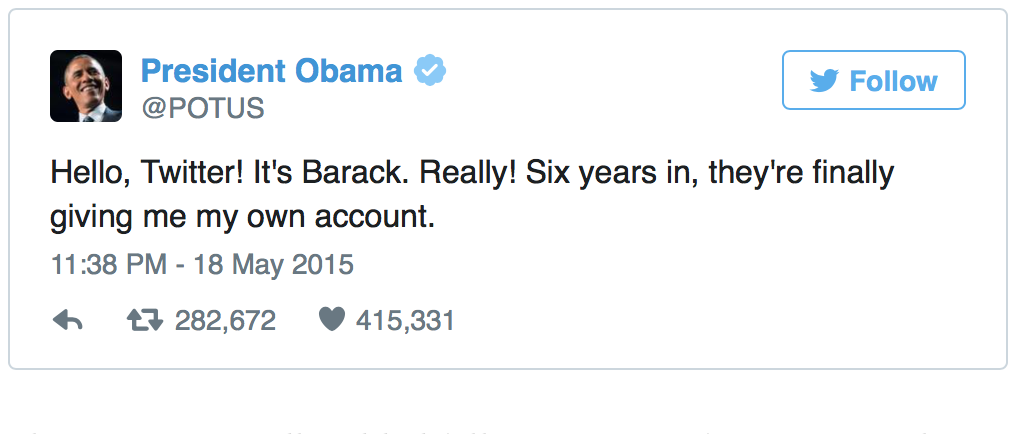
\includegraphics[width=1\textwidth]{./Pic/obama.png}
  \caption{President Obama gets his own Twitter account.}
  \end{minipage}
  \begin{minipage}[t]{.49\linewidth}
  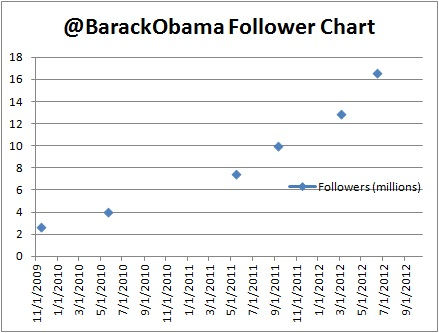
\includegraphics[width=1\textwidth]{./Pic/p5.jpg}
   %\framebox{Text}
  \caption{Graph of President Obama's follower growth.\cite{RG}}
  \label{fig:p5}
  \end{minipage}
\end{figure}
\par "Hello, Twitter! It's Barack. Really! Six years in, they're finally giving me my own account.". After President Obama opened his Facebook account, he opened his Twitter account on May 18, 2015.
\par From Figure \ref{fig:p5}, President Obama's followers has been growing rapidly over time. In our model, President Obama is one of the \textbf{\emph{Opinion Leader}}, the news that he has released is a hot and authoritative topic of concern.
\par The analysis results of this case are very consistent with our expectations, therefore, this example verifies the accuracy of our model.




\section{Strengths and Weaknesses}

\paragraph{Strengths}
\text{\\}
\begin{enumerate}%[(1)]
\renewcommand{\labelenumi}{(\theenumi)}
    \item The information network model established by us has good universality, which is suitable for all kinds of information dissemination media, and has a good time-adaptability.
    \item In our paper, we have simulated the most of the models we have built, and have been optimized to improve the stability and reliability of the model.
    \item There are many different factors that affect the complicated problem. We classify the influencing factors and put forward the quantitative indexes. At the same time, we use of examples to test the quantitative indicators which are screened out. Only in this way, can we select out the well-founded indicators.
\end{enumerate}


\paragraph{Weaknesses}
\begin{enumerate}%[(1)]
\renewcommand{\labelenumi}{(\theenumi)}
    \item We lack the research on the characteristics of the network under different media.
    \item In the \emph{\textbf{information flow and filter network}}, the feedback function of the filter has few descriptions. The noise impact in the process of information dissemination has not been taken into consideration. In addition, the age structure of the node isn't studied in-depthly.
\end{enumerate}




\newpage%另起一页书写正文
\thispagestyle{empty}%本页不遍页码
%以下是参考文献
\phantomsection%生成该页的链接
\addcontentsline{toc}{section}{\refname}
\begin{thebibliography}{}
%
% 使用指令\bibitem 构造一条参考文献.
% 具体构造方式,参考以下参考文献格式说明以及示例
% 应尽可能使用英文格式
%
\bibitem{1}
Wikipedia, Interstate compact. \url{https://en.wikipedia.org/wiki/Interstate_compact}. 2018

\bibitem{2}
Wikipedia, Factor analysis. \url{https://en.wikipedia.org/wiki/Factor_analysis#Type_of_factor_analysis}. 2018

\bibitem{3}
U.S. Energy Information Administration, State Energy Data System (SEDS): 1960-2015 (complete). \url{https://www.eia.gov/state/seds/seds-data-complete.php}. 2017

\bibitem{4}
U.S. Energy Information Administration, State Energy Data System (SEDS): 1960-2015 (complete). \url{https://www.eia.gov/state/seds/sep_use/notes/use_a.pdf}. 2017.

\bibitem{5}
Tang Mengling, Wang zhanling, and Li Zhijian. Using Model of Fcator Analysis to Calculate Weight and to Evaluate Water Quality[J]. Xingtai Vocational and Technical College, 2005.

\bibitem{L1}
U.S. Energy Information Administration, Renewable Energy Explained. \url{https://www.eia.gov/energyexplained/?page=renewable_home}. 2017



\bibitem{RE}
Stanovich K E. What Intelligence Tests Miss:The Psychology of Rational Thought[M]. Yale University Press, 2009.

\bibitem{RG}
Wikipedia, Barack Obama on social media. \url{https://en.wikipedia.org/wiki/Barack_Obama_on_social_media}. 2016


\bibitem{RF}
Pewresearch, State of the News Media 2012. \url{http://www.pewresearch.org/2012/03/19/state-of-the-news-media-2012/}. 2012

\bibitem{RK}
International Telecommunication Union, ICT Data and Statistics (IDS). \url{http://www.itu.int/ITU-D/ict/statistics/explorer/index.html}. 2016

\bibitem{RH}
Wikipedia, Quantum information science. \url{https://en.wikipedia.org/wiki/Quantum_information_science}. 2016
% etc
\end{thebibliography}




\end{document}
